\section{AE and Variational AE}

\subsubsection{Autoencoders}\label{subsubsec:autoencoders}
\textit{Autoencoders}, introduced by Rumelhart et al. in \textit{Learning internal representations by error propagation}
\cite{Rumelhart1986}, are a type of unsupervised deep neural network. They consist of two parts — an \textit{encoder} and a \textit{decoder}. The former transforms the input into a latent space, which is an informative representation. The decoder's goal is to reconstruct the inputs from the latent space \cite{Bank2020}. In other words, because of the imposed task, an autoencoder is a model mapping an input $X$ to an output $X'$ using its internal, latent representation $Z$, which is visualized in  \autoref{fig:vae-ae-architecture}. It is important, because the representation can be extracted and used in other models.

\vspace{\baselineskip}
In general, autoencoders seek to satisfy the following equation:

\begin{equation}
    argmax_{g,f}\:\mathbb{E}\left[\Delta(x, f \circ g(x))\right],
\end{equation}

\noindent where $g: \mathbb{R}^d \rightarrow \mathbb{R}^q$ is a function that the encoder is trying to learn and $f: \mathbb{R}^q \rightarrow \mathbb{R}^d$ - a function of the decoder ($d$ being the input and $q$ the latent dimension).

\vspace{\baselineskip}
What is substantial in the context of this work is that removing nonlinear operations from AE results in a latent space being identical to the one created by PCA \cite{Plaut2018}. This means that autoencoders are a generalization of PCA, and if implemented linearly, could be the PCA itself. This makes them a perfect choice for conducting experiments on them and comparing to the rest of the methods.

\begin{figure}[h]
     \centering
     \begin{subfigure}[b]{0.9\textwidth}
         \centering
         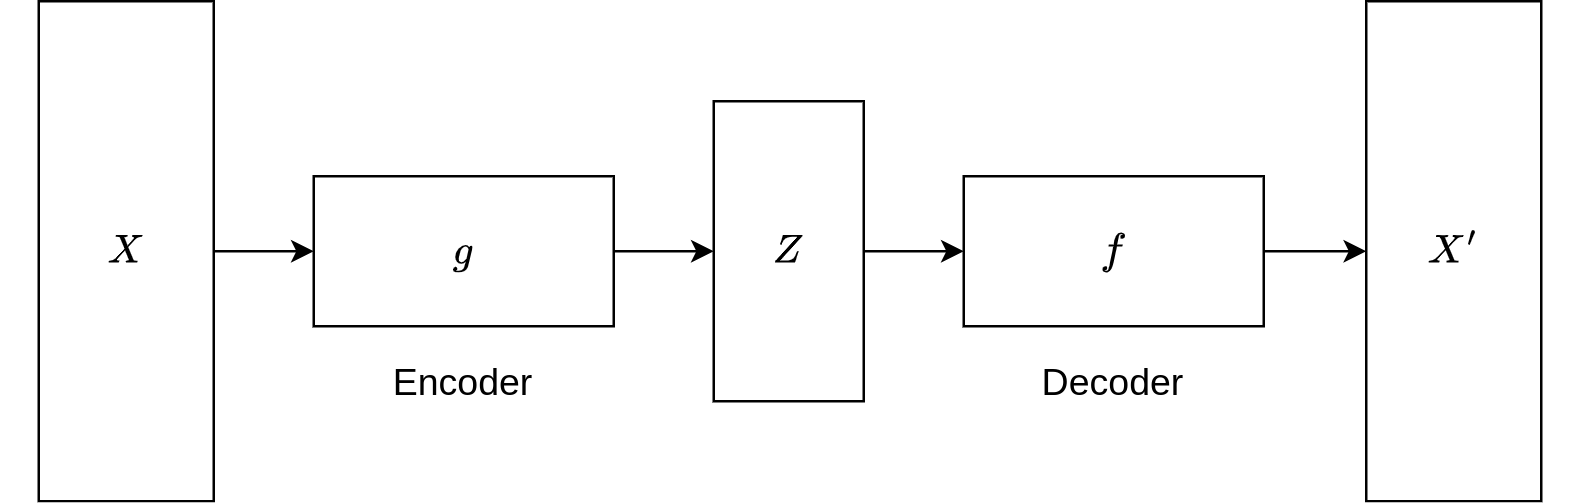
\includegraphics[width=\textwidth]{methods/img/AE_architecture.drawio.png}
         \caption{Autoencoder architecture} \label{fig:vae-ae-architecture}
     \end{subfigure} 
     \begin{subfigure}[b]{0.9\textwidth}
          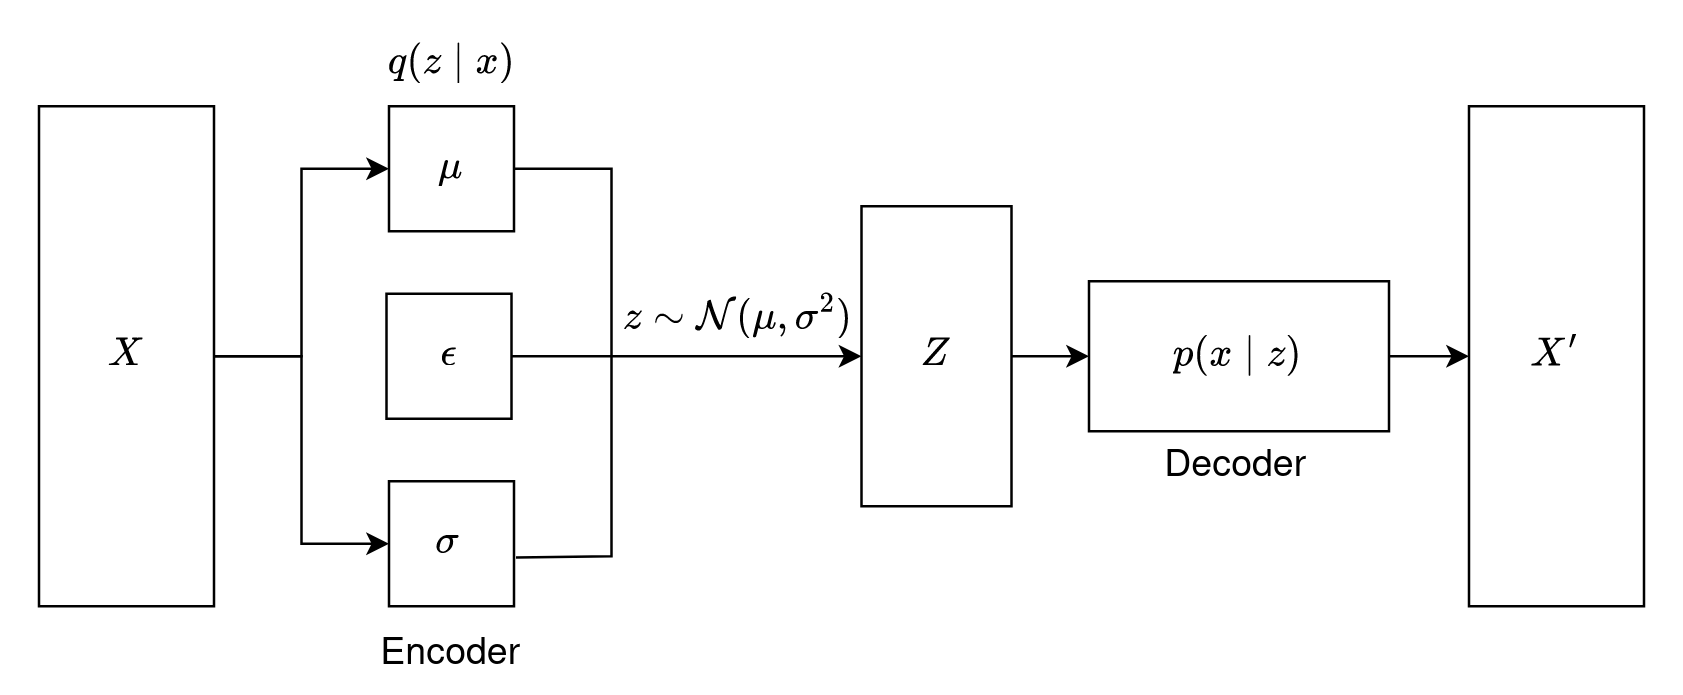
\includegraphics[width=\textwidth]{methods/img/VAE_architecture.drawio.png}
         \caption{Variational autoencoder architecture} \label{fig:vae-architecture}
     \end{subfigure} 
     \caption[Comparison of AE and VAE high-level architectures]{A comparison of Autoencoder (a) and Variational Autoencoder (b) high-level architectures.}
    \label{fig:vae-ae-architectures}
\end{figure}

\vspace{\baselineskip}
Autoencoders do face problems that can be problematic in certain applications. One of the main are being prone to overfitting, lacking explainability (due to the black-box nature), or being deterministic. While some of them can be aided by tricks or extensions (e.g., dropout for overfitting), these solutions are usually lacking in other areas.

\subsubsection{Variational autoencoders}
\textit{Variational autoencoder} (VAE) is a special example of an autoencoder \cite{Kingma2013}. Its goal remains the same; however, it is achieved not by learning functions and mapping a sample to a fixed latent vector but rather as a distribution over the latent space with a regularization term added to the reconstruction loss. This ensures the generative properties, inhibits overfitting, and improves the quality of the latent space properties.

\vspace{\baselineskip}
Introducing variational approach to autoencoders is relatively similar to the pure ELBO (see paragraph about \nameref{paragraph:vi}, especially \autoref{eq:kl}). Because both the encoder and decoder are in fact separate models, both distributions are conditional - $p(x \mid z)$ and $q(z \mid x)$ respectively, where $x$ is the data and $z$ is the latent vector. This way, the ELBO inequality (\autoref{eq:elbo-iniequality}) can be expressed as:

\begin{equation}
    \begin{split}
        \log{p(x)} & \geq \underbrace{\mathbb{E}_{z \sim q(z \mid x)} \left[ \log{p(x \mid z)}\right]}_{\textrm{reconstruction loss}} - \underbrace{D_{KL} \left[q(z \mid x) \parallel p(z) \right]}_{\textrm{posterior approximation regularization}}
    \end{split}
\end{equation}

\noindent Therefore, maximizing the ELBO and minimizing the Kullback-Leibler divergence maximizes the log-evidence.


\paragraph{Reparameterization trick}
Due to the latent variable being sampled from a distribution (instead of being deterministic), gradients cannot be backpropagated as in autoencoders. Similarly to \nameref{paragraph:bayes-by-backrop}, a reparameterization trick needs to be used. Analogously, $\epsilon$ is drawn from a fixed distribution $\mathbb{N}(0, 1)$ and $z$ takes a form of:

\begin{equation}
    z = \mu + \sigma \odot \epsilon,
\end{equation}

\noindent where $\odot$ is an element-wise product.